\section{RHEA}
Infrabel, en partenariat avec Cegelec Infra Technics et ADCIS, utilise des trains de mesure afin de vérifier les données topographiques du réseau férroviaire (\textit{cf.} Section 1.2). L'objectif d'Infrabel est d'exploiter ces données à d'autres fins, notamment l'évaluation de la quantité de ballast, en identifiant les zones présentant un excès ou un manque de ballast. Cette analyse vise à faciliter la maintenance prédictive en générant une cartographie colorée signalant les zones nécessitant une intervention. Cette approche simplifie la planification des campagnes d'entretien, actuellement basée sur des relevés pédestres. Cette section se concentre sur la présentation du projet inspirée de la documentation fournie par Cegelec \cite{RHEA}. 

\subsection{Présentation}
Infrabel envisage de mettre en place le projet RHEA pour analyser la pose du ballast, une composante importante du réseau ferrroviaire, qui soutient les rails et distribue au sol les contraintes mécaniques générées par le passage des trains. L'objectif principal de ce projet est de développer un système informatique capable de repérer les différents paramètres fonctionnels (\textit{cf.} Section 1.3) qui influencent la pose du ballast le long des voies ferroviaires.\\

Cette démarche vise à évaluer la concordance entre la pose théorique du ballast, enregistrée dans un registre chez Infrabel, et sa pose réelle obtenue grâce aux données collectées par Hyperion. L'analyse permettra de détecter d'éventuels surplus ou manques de ballast. Le résultat de cette évaluation sera utilisé pour générer une carte colorisée, facilitant ainsi la mise en oeuvre d'une maintenance prédictive ciblée. \\

L'analyse du ballast le long des rails repose sur les données fournies par plusieurs capteurs d'Hyperion ainsi que sur les données résultant de la phase de compilation. Parmi celles-ci, on peut citer :
\begin{itemize}
    \item \textbf{Les capteurs lidar 2D} \\

    
      Un Lidar 2D est un capteur équipé d'un laser et d'un élement récepteur, tel qu'une caméra (\textit{cf} Figure 4.a), permettant d'émettre un point laser sur une surface à mesurer. La lumière réfléchie par la surface atteint ensuite la caméra sous un angle particulier, ce qui permet de calculer la distance qui sépare la surface du capteur (\textit{cf} Figure 4.b \cite{triangulation}). Les distances mesurées produisent une représentation en deux dimensions de l'environnement. \\

    \begin{figure}[H]
      \centering
      \fbox{\subcaptionbox{}{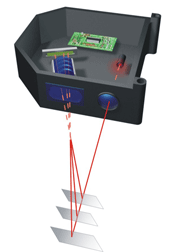
\includegraphics[width=2.35cm]{images/Lidar2D.png}}}
      \qquad % Add some space between the two subfigures
      \fbox{\subcaptionbox{}{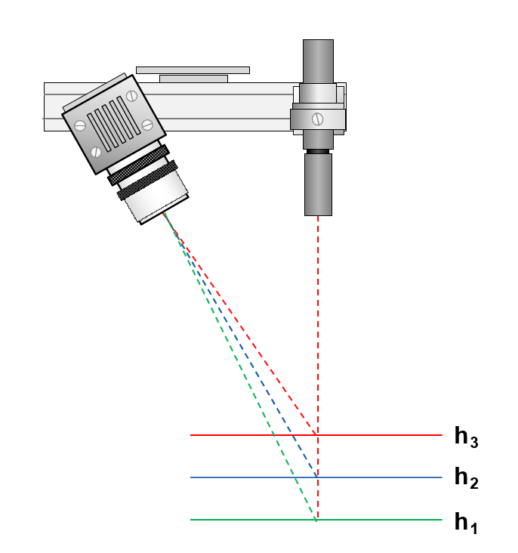
\includegraphics[width=3cm]{images/laser_triangulation.png}}}
      
      \caption{Lidar 2D}
    \end{figure}

    Quatre capteurs ont été fixés sous le plancher des trains de mesure, comme illustré sur la Figure 5,  pour recueillir les profils du sol le long d'une ligne d'observation de 4 mètres, avec une mesure effectuée tous les 4 centimètres, indépendament de la vitesse du train. L'ordonnée de ce système est centrée entre les 2 capteurs intérieurs en x et alignée sur ces deux derniers en y.


    \begin{figure}[H]
            \centering
           \fbox{ 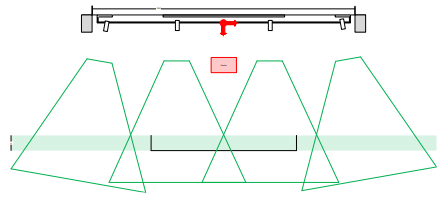
\includegraphics[width=6cm]{images/2dLidarmechaniacalimprementation.png}    }
            \caption{Méchanique d'implémentation du Lidar 2D - Cegelec \cite{RHEA}} 
        \end{figure}
    
    
    \item \textbf{Le Système de navigation inertielle} \\
    
    Le système de navigation inertielle adopté pour les trains de mesure repose sur l'Atlans-C (\textit{cf}. Figure 6). Ce système, tel que décrit par IXBlue dans sa documentation \cite{Atlans-c}, inclut un ensemble de composants comprenant un système de positionnement par satellites ou Global Navigation Satellite Systems en anglais (\gls{GNSS}), un gyroscope à fibre optique, un accéléromètre, ainsi qu'un récepteur GNSS \gls{RTK} pour des corrections en temps réel visant à atteindre une précision de l'ordre du centimètre. Cette configuration assure une détermination précise de la position, de la vitesse, de l'accélération, et de l'orientation du train, même dans des conditions complexes telles que les passages à travers des tunnels.

    \begin{figure}[H]
            \centering
           \fbox{ 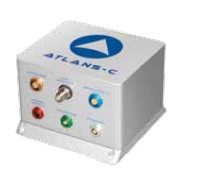
\includegraphics[width=4cm]{images/atlans-c.png}   
           }
            \caption{INS - Atlans-C \cite{Atlans-c}} 
        \end{figure}

    
    \item \textbf{La liste des éléments au sol}  \\
    
   Les profils obtenus lors de la campagne de mesure sont combinés et géolocalisés. Une image virtuelle, comme présentée dans la Figure 7, est générée à partir de ces profils, puis soumise à une intelligence artificielle chargée de repérer et d'identifier les éléments au sol, tels que les passages à niveau, les aiguillages simples ou doubles, les crocodiles, etc. Une liste exhaustive de ces éléments est ensuite produite à la fin du processus de compilation. 

    \begin{figure}[H]
            \centering
           \fbox{ 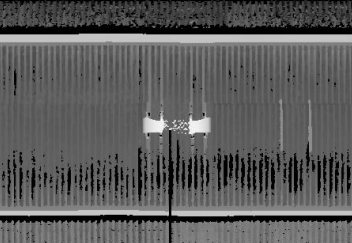
\includegraphics[width=5cm]{images/ground_list.png}   
           }
            \caption{Image virtuelle 2D - Cegelec \cite{RHEA}} 
        \end{figure}
    
\end{itemize}







\subsection{Fonctionnement}

Infrabel dispose dans ses registres d'un standard de pose du ballast qui repose sur plusieurs paramètres fonctionnels, comme introduit dans la Section 1.3 de notre étude. L'identification de ces paramètres fonctionnels permet d'établir le profil théorique du ballast, ensuite comparé avec le profil relevé, comme illustré dans la Figure 8.


\begin{figure}[H]
            \centering
           \fbox{ 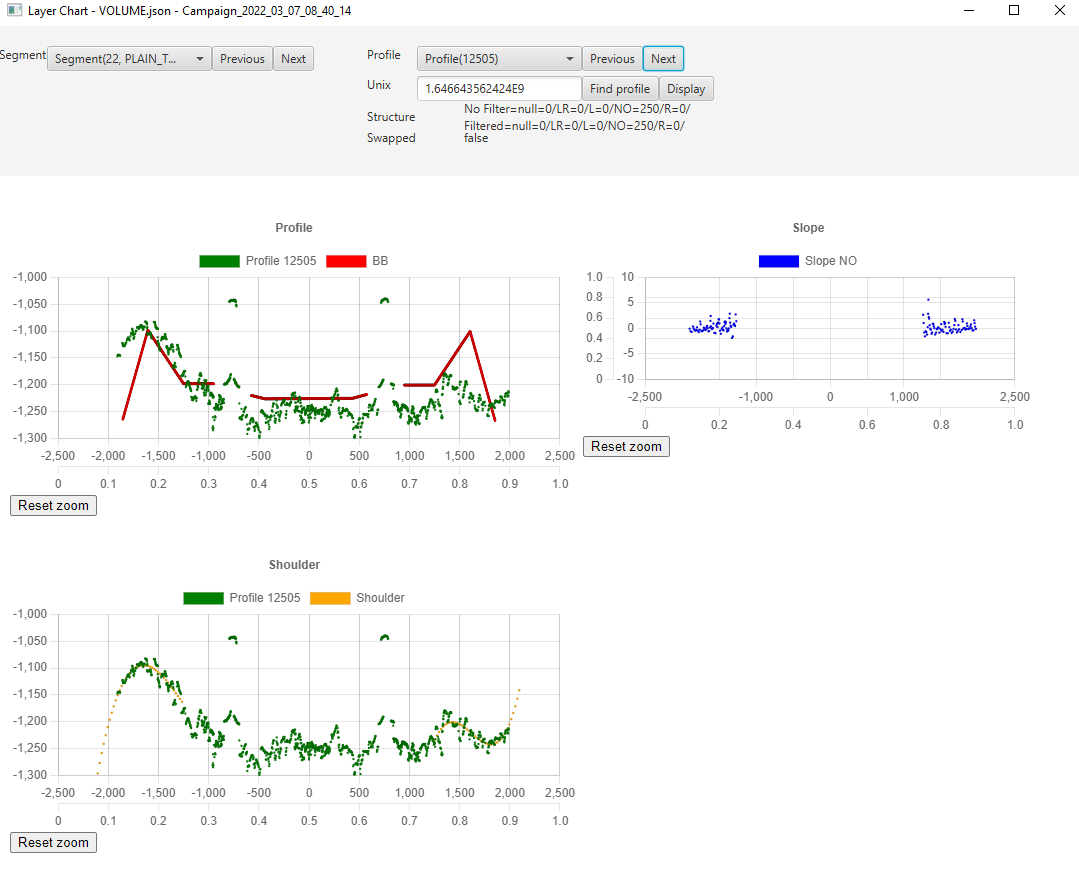
\includegraphics[width=10cm]{images/ballast-fx.PNG}   
           }
            \caption{Interface - Ballast FX } 
        \end{figure}

Cette représentation, générée à l'aide de Ballast FX, une interface créée en JavaScript dédiée à la comparaison des profils, met en évidence en rouge le profil théorique, tandis qu'en vert, un point de nuage représente le ballast réel. Cette visualisation permet d'identifier d'éventuelles variations, signalées par des zones où le ballast diffère du profil théorique. Les points verts situés au-delà de la ligne rouge pourraient signaler un excès de ballast, tandis que des zones sans points pourraient révéler un manque de ballast. \\

    \begin{figure}[H]
            \centering

           \fbox{ 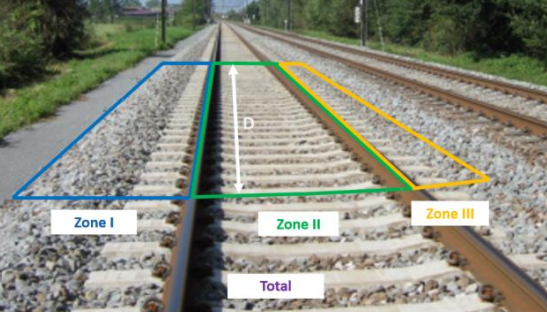
\includegraphics[width=8cm]{images/zones.png}   
           }
            \caption{Zone 1, 2 et 3 - Cegelec \cite{RHEA}} 
        \end{figure}
    


L'analyse du ballast est réalisé sur des segments de voie, qui représentent de petites fractions de la voie présentant des caractéristiques communes sur toute leur longueur. Cette analyse repose sur trois zones distinctes (\textit{cf.} Figure 9) pour identifier le manquement ou les excès de ballast. Ces zones sont : 


\begin{itemize}
    \item Zone 1 correspond à la partie gauche du rail gauche ;
    \item Zone 2 se situe entre les rails ;
    \item Zone 3 concerne la partie droite du rail droit.
\end{itemize}

\noindent Une fois cette analyse effectuée, les zones requérant une intervention sont enregistrées dans un fichier JSON au format GeoJSON. Ce fichier peut ensuite être intégré dans un système d'information géographique, tel que le logiciel QGIS (Quantum Geographic Information System), afin de générer une cartographie où les zones nécessitant une intervention sont visualisées en couleur, comme démontré dans la Figure 10.\\
\begin{figure}[H]
            \centering
           \fbox{ 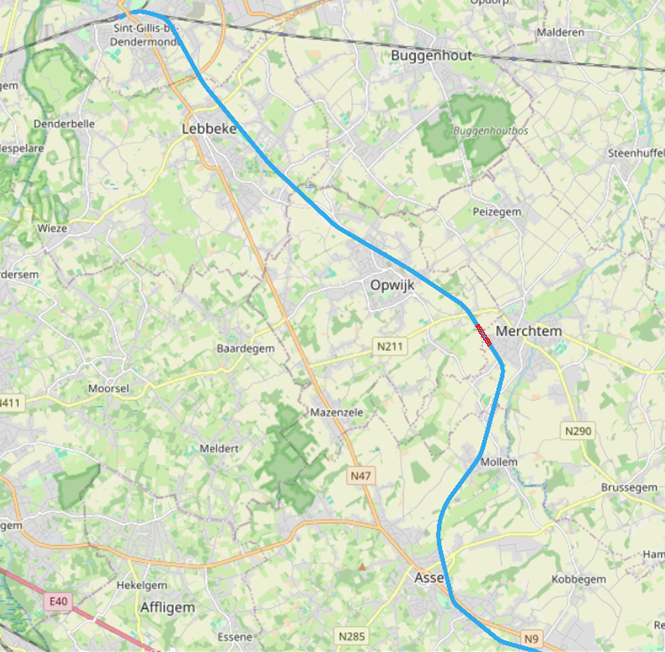
\includegraphics[width=6cm]{images/QGIS.PNG}   
           }
            \caption{Cartographie des zones nécessitant une intervention - QGIS } 
        \end{figure}

Cette cartographie offre une visualisation claire des zones spécifiques où des ajustements sont nécessaires, facilitant ainsi la planification des travaux de maintenance et contribuant à la gestion de la qualité du ballast sur le réseau ferroviaire.


\subsection{Définition du problème}


Pour effectuer l'analyse du ballast, l'accès aux données collectées au cours d'une campagne de mesure est essentielle. Ces données, stockées dans un fichier appelé *.campaign, peuvent être récupérées à l'aide des web services intégrés dans le code Java. Elles sont indispensables pour comparer la pose réelles et la pose théorique du ballast.\\
\newpage

\noindent La forme théorique du ballast est déterminée en fonction de divers paramètres fonctionnels (\textit{cf.} Figure 11). Il est impératif d'identifier ces paramètres pour sélectionner la forme théorique adéquate et conduire ainsi une analyse du ballast.\\

\begin{figure}[H]
            \centering
           \fbox{ 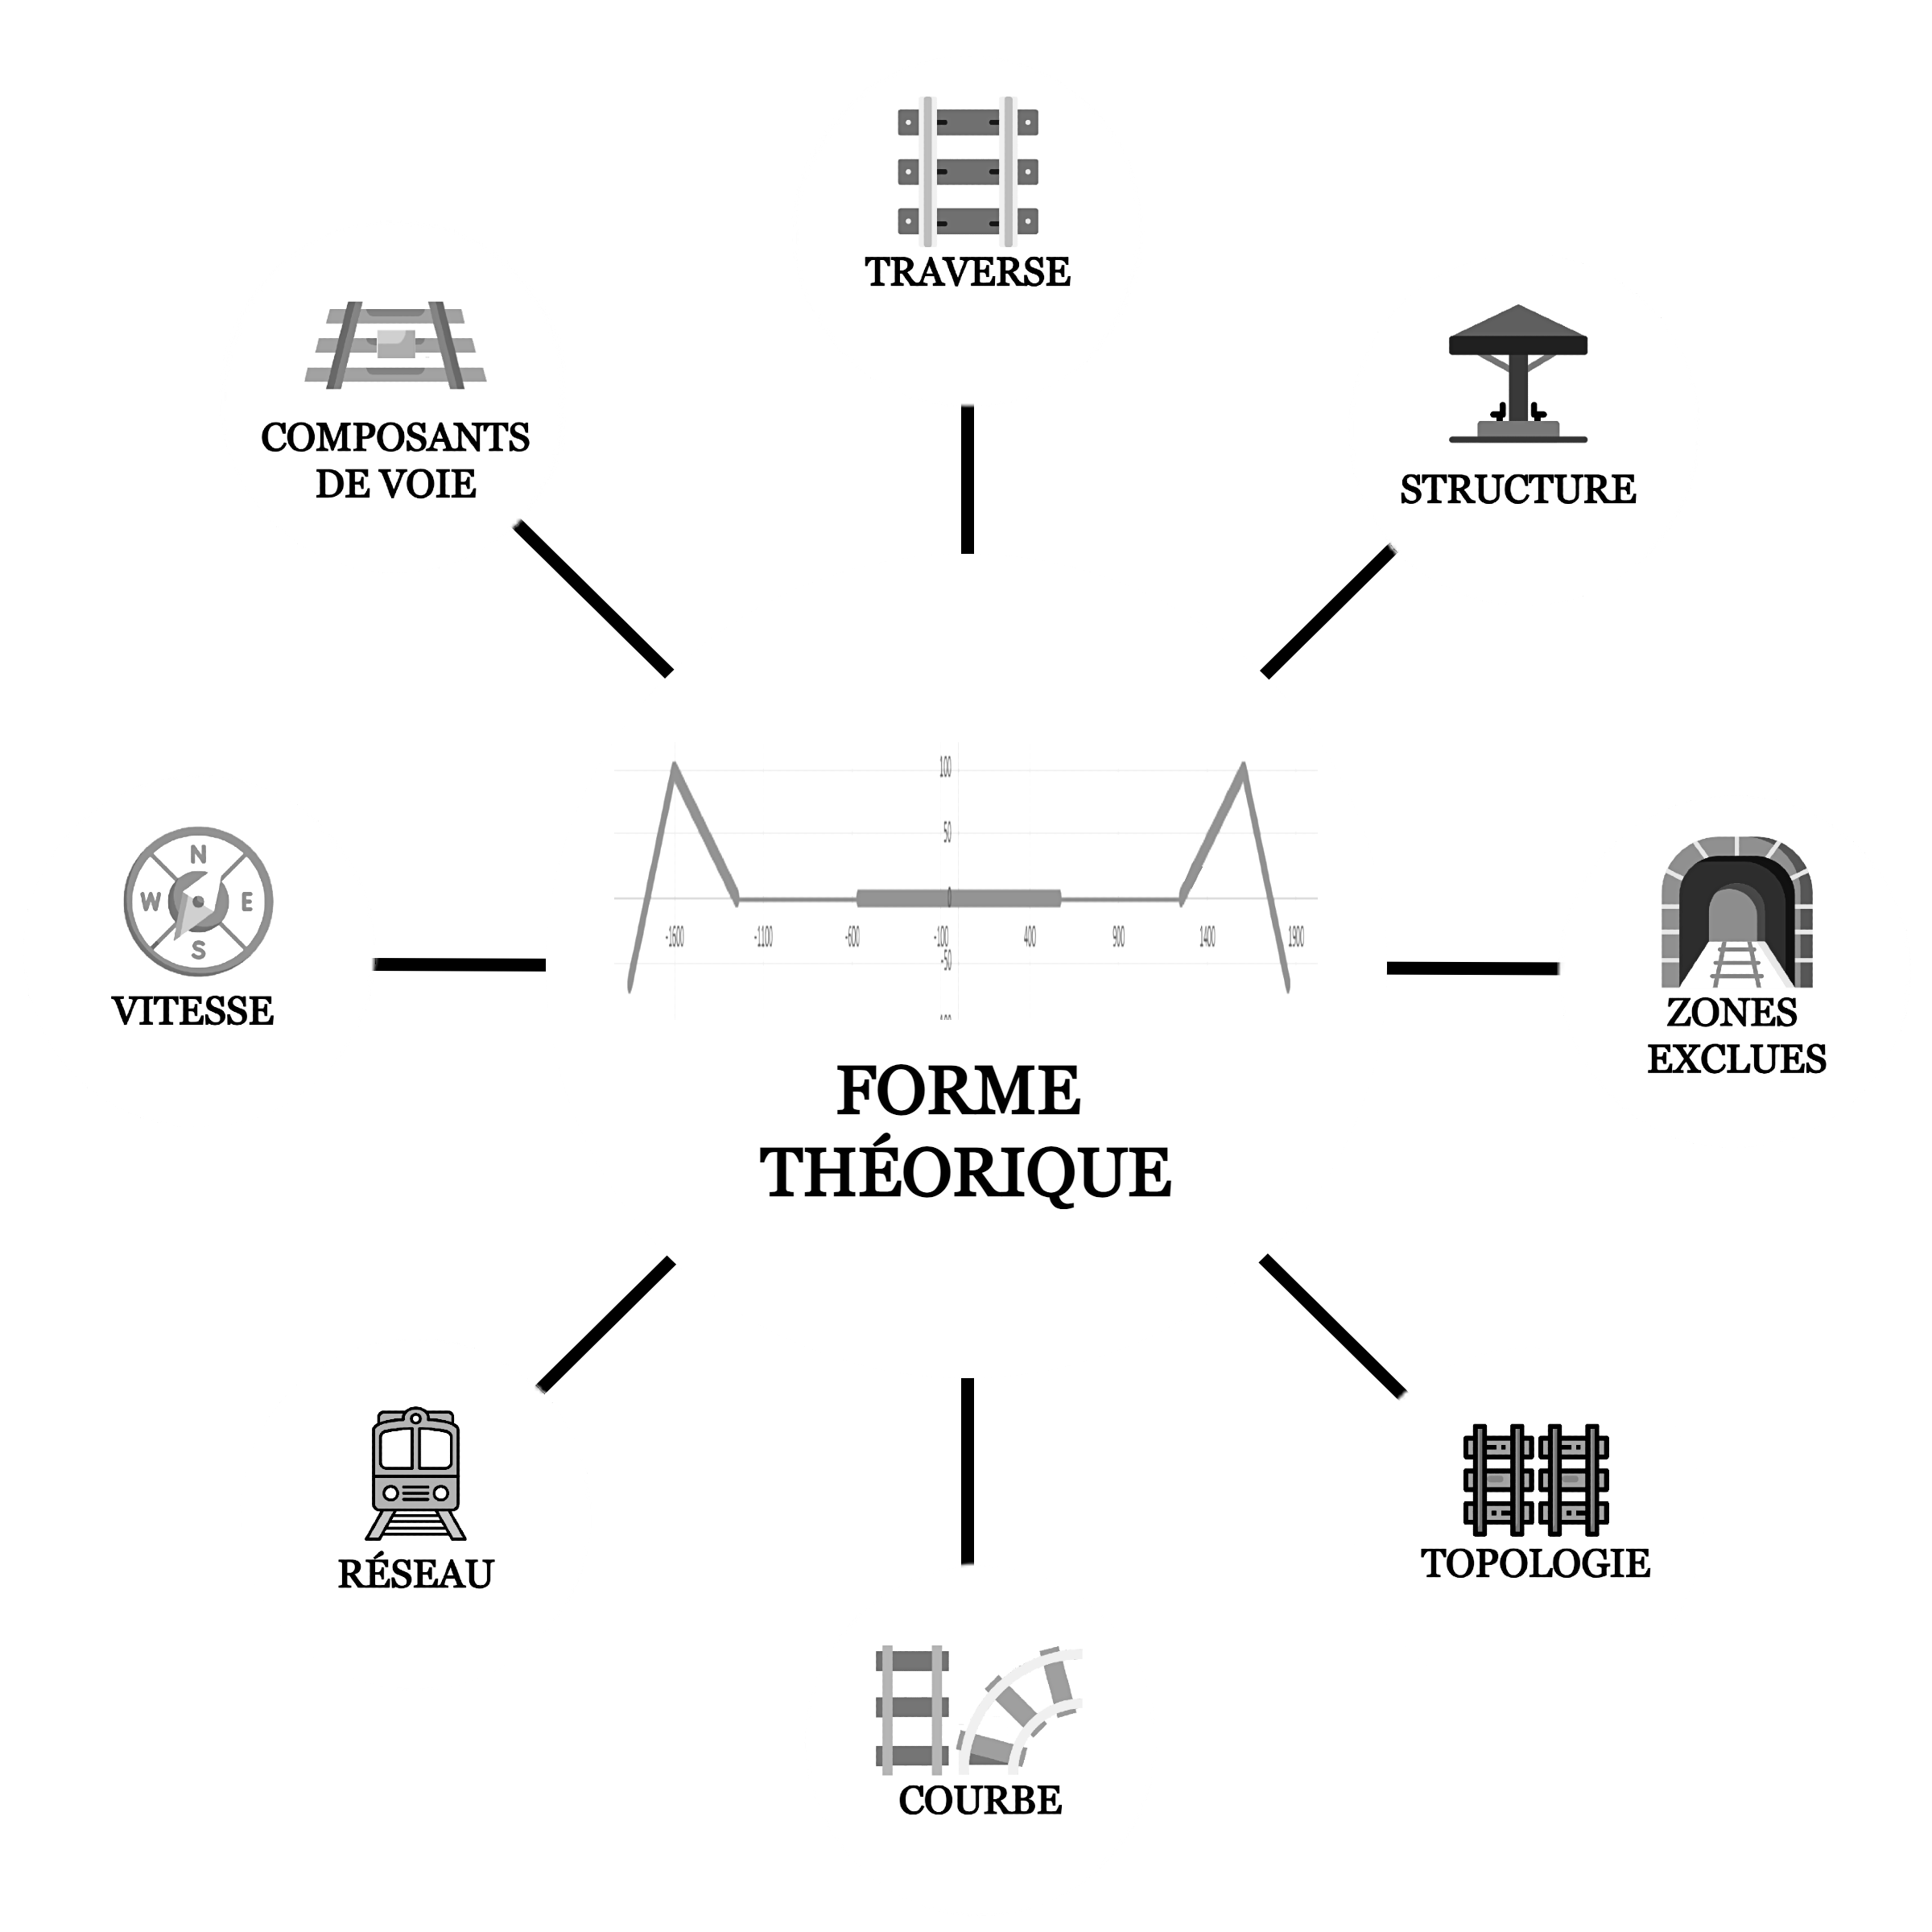
\includegraphics[width=7cm]{images/PARAMFONC1.png}   
           }
            \caption{Paramètres fonctionels } 
        \end{figure}


\noindent Certains paramètres, tels que la vitesse, le type de réseau, la structure, les zones exclues et les composantes de voies, sont déjà identifiés et constituent une base de données essentielle pour l'analyse. \\


\noindent Cependant, d'autres paramètres tels que le type de traverse et la topologie nécessitent une étude approfondie, et ces éléments constituent les objectifs principaux de ce stage, comme précisé dans la Section 1.3. \\


\noindent En ce qui concerne le type de traverse, une première approche de détection repose sur une méthode mathématique qui fonctionne de manière raisonnable, c'est-à-dire qui identfie correctement les traverses. Toutefois, certaines limitations se manifestent dans des conditions spécifiques. Les détails de cette approche, ainsi que ses limitations, sont couverts dans la Section 4. Pour remédier à ces limitations, la Section 5 présente une analyse basée sur des modèles d'intelligence artificielle. Cette analyse permet de comparer les deux approches afin de déterminer la plus performante  pour la détection du type de traverse. \\

 \noindent La détection de la topologie repose aussi sur une approche d'IA et elle sera étudié ultérieurement si le temps le permet. 
% montrer une exemple de la carte cartographié, d'une comparaison entre le ballast et le profil théorique. parler des différents paramètre fonctionnelles qui doivent être derterminer au préalable. Dire par exemple que la traverse est en cours d'études car c'est la cas de mon stage que la vitesse on l'obtient directement, parler de la topologie de la voie, les grounds element on a déjà donc çava comme le ETCS ou le simple track. Parler qu'on doit identifier si il y a des voies à proximité des voies adjacentes. 


% Parler de comment les enregistrement sont fait, tous les 4 centimètres etc
% COmment l'analyse du profil se fait 

% Parler des données récolter, quelles sont ses données sous quelles formes sont-elles ? 


\subsection{Objectif}
L'objectif principal du projet, comme énoncé dans la Section 1.3, est d'assurer une identification précise des paramètres fonctionnels liés à la pose du ballast, tels que le type de traverse ou la topologie, afin de mettre en place un système de maintenance prédictive pour les voies ferrées. Ceci sera réalisé en se basant sur l'analyse des données collectées par des capteurs au niveau du sol. \\

Le projet sera divisé en trois parties, chacune représentant un aspect distinct des objectifs du stage, et suivra le schéma suivant.
\begin{enumerate}
    \item Collecte des données : La première étape du projet consiste à collecter les données en examinant leur format et leur disposition, afin d'extraire celles qui seront utiles pour l'analyse du ballast.

    \item Exploration des données et développement de modèles d'IA : Ensuite, les données seront explorées en utilisant différentes méthodes d'IA pour identifier les profils des traverses ferroviaires. Cela impliquera de définir une stratégie de détection et de choisir les modèles de classification appropriés.
\newpage
    \item Évaluation et intégration : Après avoir examiné ces méthodes, nous évaluerons la précision des modèles afin d'atteindre les objectifs d'identification les plus précis possible. Ensuite, nous étudierons les possibilités d'intégrer les outils d'IA développés en Python dans l'écosystème Java, en explorant diverses approches telles que l'utilisation d'API, de scripts ou d'autres méthodes pour déterminer la meilleure méthode d'intégration.
\end{enumerate}



